\documentclass[12pt,a4paper]{article}

% ─── Page Layout ───────────────────────────────────────────────────────────────
\usepackage[a4paper, margin=0.8in, headheight=14pt]{geometry}

% ─── Fonts (XeLaTeX) ───────────────────────────────────────────────────────────
\usepackage{fontspec}
\usepackage{unicode-math}
\setmainfont{TeX Gyre Pagella}
\setmonofont[Scale=0.88]{TeX Gyre Cursor}
\setmathfont{Latin Modern Math}

% ─── Packages ──────────────────────────────────────────────────────────────────
\usepackage{xcolor}
\usepackage{colortbl}
\usepackage{titlesec}
\usepackage{enumitem}
\usepackage{tabularx}
\usepackage{longtable}
\usepackage{booktabs}
\usepackage{array}
\usepackage{amsmath}
\usepackage{tikz}
\usetikzlibrary{shapes.geometric, arrows.meta, positioning, calc, fit, decorations.pathreplacing, patterns}
\usepackage{tcolorbox}
\tcbuselibrary{skins, breakable}
\usepackage{hyperref}
\usepackage{fancyhdr}
\usepackage{graphicx}
\usepackage{microtype}
\hyphenpenalty=10000
\exhyphenpenalty=10000
\sloppy
\usepackage{caption}
\usepackage{setspace}
\usepackage{multirow}
\usepackage{tocloft}

% ─── Q&A helper ────────────────────────────────────────────────────────────────
\newcommand{\Q}[1]{\textbf{#1}\par\noindent\ignorespaces}

% ─── Colour Palette ────────────────────────────────────────────────────────────
\definecolor{myred}{RGB}{196,30,58}
\definecolor{mydark}{RGB}{30,30,50}
\definecolor{mygreen}{RGB}{14,120,80}
\definecolor{myteal}{RGB}{0,130,140}
\definecolor{myamber}{RGB}{180,100,0}
\definecolor{mypurple}{RGB}{100,30,160}
\definecolor{mygray}{RGB}{246,247,249}
\definecolor{mgframe}{RGB}{180,185,200}
\definecolor{watermark}{RGB}{145,150,170}
\definecolor{hdrred}{RGB}{250,232,235}
\definecolor{hdrgreen}{RGB}{220,244,233}
\definecolor{hdrteal}{RGB}{220,242,244}
\definecolor{hdramber}{RGB}{253,242,215}
\definecolor{hdrpurple}{RGB}{238,228,255}
\definecolor{hdrgray}{RGB}{238,240,245}

% ─── Section Formatting ────────────────────────────────────────────────────────
\titleformat{\section}
  {\large\bfseries\color{myred}}{\thesection.}{0.5em}{}
  [\vspace{1pt}{\color{myred}\rule{\linewidth}{0.8pt}}]
\titleformat{\subsection}
  {\normalsize\bfseries\color{myteal}}{\thesubsection}{0.5em}{}
\titlespacing*{\section}{0pt}{18pt}{7pt}
\titlespacing*{\subsection}{0pt}{11pt}{4pt}

% ─── Paragraph ─────────────────────────────────────────────────────────────────
\setlength{\parindent}{0pt}
\setlength{\parskip}{4pt}

% ─── TOC Styling ───────────────────────────────────────────────────────────────
\renewcommand{\cfttoctitlefont}{\large\bfseries\color{myred}}
\renewcommand{\cftaftertoctitle}{\par\noindent{\color{myred}\rule{\linewidth}{0.8pt}}}
\setlength{\cftbeforetoctitleskip}{0pt}
\setlength{\cftaftertoctitleskip}{6pt}
\renewcommand{\cftsecfont}{\normalsize\bfseries\color{mydark}}
\renewcommand{\cftsecpagefont}{\normalsize\bfseries\color{mydark}}
\renewcommand{\cftsecleader}{\cftdotfill{\cftdotsep}}
\setlength{\cftbeforesecskip}{7pt}
\renewcommand{\cftsubsecfont}{\small\color{mydark}}
\renewcommand{\cftsubsecpagefont}{\small\color{mydark}}
\setlength{\cftbeforesubsecskip}{3pt}
\setlength{\cftsubsecindent}{1.4em}

% ─── Table helpers ─────────────────────────────────────────────────────────────
\renewcommand{\arraystretch}{1.45}
\setlength{\tabcolsep}{6pt}
\arrayrulecolor{mydark}
\newcolumntype{B}[1]{>{\small\bfseries\raggedright\arraybackslash}m{#1}}
\newcolumntype{Y}{>{\small\raggedright\arraybackslash}X}
\renewcommand{\tabularxcolumn}[1]{m{#1}}

% ─── Header / Footer ───────────────────────────────────────────────────────────
\pagestyle{fancy}
\fancyhf{}
\fancyhead[L]{\small\color{myred}\textbf{BS-B401}\;\color{mydark}--- Biology for Engineers}
\fancyhead[R]{\small\color{myteal}\textbf{Module 8 Notes}}
\fancyfoot[C]{\small\color{mydark}\thepage}
\fancyfoot[R]{\small\color{watermark}\textit{\copyright\ Biraj Sarkar (CGEC)}}
\renewcommand{\headrulewidth}{0.5pt}
\renewcommand{\footrulewidth}{0.3pt}

% ─── Hyperref ──────────────────────────────────────────────────────────────────
\hypersetup{
  colorlinks=true, linkcolor=myteal, urlcolor=myteal,
  pdfauthor={Biraj Sarkar (CGEC)},
  pdftitle={BS-B401 --- Module 8 Notes: Metabolism}
}

% ─── tcolorbox styles ──────────────────────────────────────────────────────────
\tcbset{
  tikzbox/.style={
    colback=mygray, colframe=mgframe, boxrule=0.6pt, arc=4pt,
    left=8pt, right=8pt, top=6pt, bottom=6pt,
    colbacktitle=mgframe, coltitle=mydark, fonttitle=\small\bfseries
  },
  defbox/.style={
    colback=hdrgreen, colframe=mygreen, boxrule=0.8pt, arc=4pt,
    left=9pt, right=9pt, top=6pt, bottom=6pt,
    colbacktitle=mygreen, coltitle=white, fonttitle=\small\bfseries
  },
  formulabox/.style={
    colback=hdrteal, colframe=myteal, boxrule=0.8pt, arc=4pt,
    left=9pt, right=9pt, top=7pt, bottom=7pt,
    colbacktitle=myteal, coltitle=white, fonttitle=\small\bfseries
  },
  examplebox/.style={
    colback=hdramber, colframe=myamber, boxrule=0.8pt, arc=4pt,
    left=9pt, right=9pt, top=6pt, bottom=6pt,
    colbacktitle=myamber, coltitle=white, fonttitle=\small\bfseries
  },
  masonbox/.style={
    colback=hdrpurple, colframe=mypurple, boxrule=0.8pt, arc=4pt,
    left=9pt, right=9pt, top=6pt, bottom=6pt,
    colbacktitle=mypurple, coltitle=white, fonttitle=\small\bfseries
  },
  exambox/.style={
    colback=hdrpurple, colframe=mypurple, boxrule=1pt, arc=5pt,
    left=10pt, right=10pt, top=8pt, bottom=8pt,
    colbacktitle=mypurple, coltitle=white, fonttitle=\bfseries,
    breakable, title after break={\textbf{Frequently Asked / Viva Questions (contd.)}}
  }
}
\tcbset{breakable}
\tcbset{after={\par\color{black}}}

% ─── TikZ styles ───────────────────────────────────────────────────────────────
\tikzset{
  block/.style={rectangle, draw=myteal, fill=hdrteal,
    text width=2.4cm, align=center, minimum height=0.95cm,
    font=\small, rounded corners=3pt, line width=0.7pt},
  redblock/.style={rectangle, draw=myred, fill=hdrred,
    text width=2.4cm, align=center, minimum height=0.95cm,
    font=\small, rounded corners=3pt, line width=0.7pt},
  amberblock/.style={rectangle, draw=myamber, fill=hdramber,
    text width=2.4cm, align=center, minimum height=0.95cm,
    font=\small, rounded corners=3pt, line width=0.7pt},
  sumjunc/.style={circle, draw=myamber, fill=hdramber,
    minimum size=0.62cm, font=\small, line width=0.8pt},
  arrow/.style={-Stealth, thick, color=mydark},
  redarrow/.style={-Stealth, thick, color=myred},
  line/.style={thick, color=mydark}
}

\begin{document}

% ─── Title Page ───────────────────────────────────────────────────────────────
\begin{center}
  {\LARGE\bfseries\color{myred} BS-B401 --- Biology for Engineers}\\[5pt]
  {\normalsize\color{mydark} Semester IV \quad$\bullet$\quad 2L:1T:0P \quad$\bullet$\quad 3 Credits}\\[3pt]
  {\normalsize\color{myteal}\textbf{Module 8 Exam Notes: Metabolism}}\\[3pt]
  {\small\color{mydark} CGEC \;$|$\; B.Tech ECE (2023--27) \;$|$\; \textit{Biraj Sarkar}}
\end{center}
\vspace{2pt}
\noindent{\color{myred}\rule{\linewidth}{1.5pt}}
\vspace{2pt}

\hypersetup{linkcolor=mydark}
\tableofcontents
\hypersetup{linkcolor=myteal}
\newpage

\section{Metabolism}
\subsection{Thermodynamics in an open biological system}
\begin{tcolorbox}[defbox, title={Metabolism}]
Metabolism is the network of chemical reactions that supplies materials and energy. Catabolic reactions break down molecules and often release usable free energy. Anabolic reactions build molecules and generally need energy input. Cells exchange matter and energy with their surroundings.
\end{tcolorbox}

\par\vspace{5pt}
\begingroup
\setlength{\extrarowheight}{1pt}
\noindent\begin{tabularx}{\linewidth}{|B{3.25cm}|Y|Y|}
\hline
\textbf{Description} & \textbf{Criterion} & \textbf{Meaning} \\ \hline
Exothermic / endothermic & $\Delta H<0$ / $\Delta H>0$. & Heat released or absorbed at constant pressure. \\ \hline
Exergonic / endergonic & $\Delta G<0$ / $\Delta G>0$. & Forward direction is thermodynamically favourable or unfavourable under the stated conditions. \\ \hline
Equilibrium & $\Delta G=0$ and $Q=K_{\mathrm{eq}}$. & No net change. Forward and reverse processes balance. \\ \hline
\end{tabularx}\par
\endgroup
\begin{tcolorbox}[formulabox, title={Actual and standard free energy}]
At uniform temperature and pressure,
\[
\begin{aligned}
\Delta G&=\Delta H-T\Delta S,\\
\Delta G&=\Delta G^\circ+RT\ln Q,\\
\Delta G^\circ&=-RT\ln K_{\mathrm{eq}} .
\end{aligned}
\]
$Q$ is the current activity ratio, whereas $K_{\mathrm{eq}}$ is its equilibrium value. Use kelvin for $T$ and consistent energy units. In biochemistry, a prime as in $\Delta G^{\circ\prime}$ denotes a transformed standard state, often at specified pH, with the corresponding transformed quotient and equilibrium constant.
\end{tcolorbox}

\begin{tcolorbox}[examplebox, title={Calculate a standard free energy}]
At $298\,\mathrm K$, let $K_{\mathrm{eq}}=100$. Then
\[
\begin{aligned}
\Delta G^\circ
  &=-(8.314)(298)\ln(100)\,\mathrm{J\,mol^{-1}}\\
  &\approx -11.4\,\mathrm{kJ\,mol^{-1}} .
\end{aligned}
\]
The standard value favours products. Under actual conditions, use $Q$. If $Q>K_{\mathrm{eq}}$, the forward $\Delta G$ is positive. \textbf{Spontaneity.} A negative actual $\Delta G$ favours forward change. The activation barrier affects its speed.
\end{tcolorbox}

\subsection{ATP, coupling and energy charge}
\begin{itemize}[leftmargin=*, itemsep=3pt, topsep=4pt]
  \item \textbf{Energy currency.} ATP hydrolysis to ADP and inorganic phosphate can drive work or synthesis when reactions are coupled.
  \item \textbf{Add the free-energy changes.} A coupled process is favourable when its combined $\Delta G$ is negative. A shared intermediate or energy-transferring enzyme is needed to link the reactions.
  \item \textbf{Explain hydrolysis.} Free energy depends on the total reactant and product states. Bond breaking alone costs energy. Products can be favoured by factors such as solvation and resonance.
\end{itemize}
\begin{tcolorbox}[examplebox, title={Energy charge of an adenylate pool}]
Energy charge measures adenylates on a scale from 0 (all AMP) to 1 (all ATP):
\[
\begin{aligned}
\mathrm{EC}
 &=\frac{[\mathrm{ATP}]+\frac12[\mathrm{ADP}]}{[\mathrm{ATP}]+[\mathrm{ADP}]+[\mathrm{AMP}]}\\
 &=\frac{3+\frac12(1)}{3+1+1}=0.70
\end{aligned}
\]
for ATP, ADP and AMP concentrations of 3, 1 and 1 mM. The ratio has no units. A rise in ATP relative to AMP raises the charge.
\end{tcolorbox}

\section{Glucose Breakdown and Photosynthesis}
\subsection{Aerobic oxidation of glucose}
\begin{tcolorbox}[formulabox, title={Overall carbon and oxygen balance}]
\[
\mathrm{C_6H_{12}O_6+6O_2\to6CO_2+6H_2O}.
\]
The equation describes the net outcome. The stages transfer energy into ATP and reduced electron carriers.
\end{tcolorbox}

\par\vspace{5pt}
\begingroup
\setlength{\extrarowheight}{1pt}
\noindent\begin{tabularx}{\linewidth}{|B{3.5cm}|Y|Y|}
\hline
\textbf{Stage} & \textbf{Main events per glucose} & \textbf{Where it occurs in a typical eukaryotic cell} \\ \hline
Glycolysis & One glucose yields two pyruvate, net two ATP and two NADH. The energy-investment phase spends ATP before the payoff phase makes more. & Cytosol. \\ \hline
Pyruvate oxidation & Two pyruvate produce two acetyl-CoA, two carbon dioxide and two NADH. & Mitochondrial matrix. \\ \hline
Krebs cycle & Two acetyl groups yield four carbon dioxide, six NADH, two FADH2 and two ATP/GTP equivalents. Oxaloacetate is regenerated. & Mainly mitochondrial matrix. \\ \hline
Electron transport and ATP synthesis & Electrons from reduced carriers ultimately reduce oxygen to water. The proton gradient drives ATP synthase. & Inner mitochondrial membrane. \\ \hline
\end{tabularx}\par
\endgroup
\begin{tcolorbox}[masonbox, title={Keep the roles separate}]
Glycolysis does not require oxygen directly. Oxygen supports aerobic oxidation as the terminal electron acceptor in the respiratory chain. Most ATP in typical aerobic oxidation comes from oxidative phosphorylation, and the exact overall yield can vary.
\end{tcolorbox}

\subsection{Track carbon and electron carriers without memorising an ATP total}
\begin{tcolorbox}[tikzbox, title={Carbon flow during aerobic glucose oxidation}]
\centering
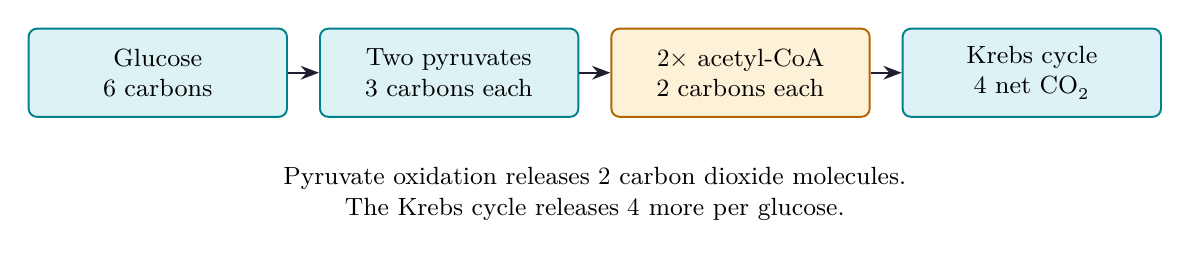
\begin{tikzpicture}[every node/.style={font=\small},
  carbonstep/.style={text width=3cm,minimum height=1.12cm,inner sep=4pt}]
\node[block,carbonstep] (a) at (0,0) {Glucose\\6 carbons};
\node[block,carbonstep] (b) at (3.7,0) {Two pyruvates\\3 carbons each};
\node[amberblock,carbonstep] (c) at (7.4,0) {$2\times$ acetyl-CoA\\2 carbons each};
\node[block,carbonstep] (d) at (11.1,0) {Krebs cycle\\4 net $\mathrm{CO_2}$};
\draw[arrow] (a)--(b);
\draw[arrow] (b)--(c);
\draw[arrow] (c)--(d);
\node[align=center] at (5.55,-1.54) {Pyruvate oxidation releases $2$ carbon dioxide molecules.\\The Krebs cycle releases $4$ more per glucose.};
\end{tikzpicture}\par
\end{tcolorbox}

\begin{itemize}[leftmargin=*, itemsep=2pt]
  \item \textbf{Glycolysis.} Glucose splits into two three-carbon molecules, with no net carbon dioxide release. Substrate-level phosphorylation transfers phosphate directly to ADP.
  \item \textbf{Pyruvate oxidation and the cycle.} Pyruvate oxidation drops one carbon per pyruvate. The cycle releases two carbon dioxide molecules per turn while regenerating oxaloacetate. This is a net balance, since newly entered carbon atoms need not be the ones released in the first turn.
  \item \textbf{Oxidative phosphorylation.} NADH and FADH2 carry reducing equivalents. Electron transfer creates a proton gradient, and flow through ATP synthase couples that gradient to ATP formation. Oxygen is the terminal electron acceptor.
\end{itemize}

\subsection{Photosynthesis builds carbohydrate}
\begin{enumerate}[leftmargin=*, itemsep=3pt, topsep=4pt]
  \item \textbf{Capture light.} In oxygenic photosynthesis, light reactions in thylakoid membranes generate ATP and reducing power in the form of NADPH. Splitting water supplies electrons and releases oxygen.
  \item \textbf{Fix carbon.} The Calvin cycle uses carbon dioxide, ATP and NADPH to make triose phosphate and regenerate its carbon dioxide acceptor. Glucose and other carbohydrates can be assembled from the triose products.
  \item \textbf{Read the net equation.} A simplified net representation is
 \[
 \mathrm{6CO_2+6H_2O \xrightarrow{light} C_6H_{12}O_6+6O_2}.
 \]
 The oxygen released in oxygenic photosynthesis originates from water. The equation summarises the energy-consuming carbon synthesis.
\end{enumerate}
\par\vspace{5pt}
\begingroup
\setlength{\extrarowheight}{1pt}
\noindent\begin{tabularx}{\linewidth}{|B{3.45cm}|Y|Y|}
\hline
\textbf{Pathway} & \textbf{Carbon direction} & \textbf{Energy relationship} \\ \hline
Aerobic respiration & Reduced carbon in glucose is oxidised to carbon dioxide. & Energy-yielding overall, with useful energy transferred to ATP. \\ \hline
Oxygenic photosynthesis & Carbon dioxide is reduced to carbohydrate precursors. & Light energy is captured, then ATP and NADPH help drive carbon fixation. \\ \hline
\end{tabularx}\par
\endgroup

\subsection{Work the energy balance in either direction}
\begin{tcolorbox}[examplebox, title={One uphill reaction coupled to ATP hydrolysis}]
Suppose a biosynthetic step has $\Delta G=+14\,\mathrm{kJ\,mol^{-1}}$ and its coupled ATP hydrolysis has $\Delta G=-30\,\mathrm{kJ\,mol^{-1}}$ under the same stated conditions. Add changes in the same stoichiometric amount:
\[
\Delta G_{\mathrm{net}}=14-30=-16\,\mathrm{kJ\,mol^{-1}}.
\]
This predicts favourable forward change when an actual coupling mechanism links the events.
\end{tcolorbox}

\begin{itemize}[leftmargin=*, itemsep=2pt]
  \item \textbf{Photosynthetic reducing power.} Light reactions produce NADPH, which supplies electrons for reducing fixed carbon, as well as ATP to drive reactions in the Calvin cycle.
  \item \textbf{Carbon-fixation budget.} Fixing three carbon dioxide molecules to yield one net three-carbon triose phosphate uses nine ATP and six NADPH in the standard Calvin cycle count. Two net triose phosphates provide the six carbons needed for a hexose equivalent.
  \item \textbf{Why the cycles differ.} The Krebs cycle oxidises acetyl groups and regenerates oxaloacetate. The Calvin cycle uses chemical energy to fix carbon and regenerates the carbon dioxide acceptor.
\end{itemize}

\textbf{Reading.} \href{https://pubmed.ncbi.nlm.nih.gov/4972613/}{Atkinson's original adenylate energy-charge paper}.

\newpage
\begin{center}
  {\large\bfseries\color{myred} Quick Revision --- Module 8}\\[3pt]
  {\small\color{mydark} Metabolism $|$ BS-B401}
\end{center}
\noindent{\color{myred}\rule{\linewidth}{1.2pt}}\par\vspace{4pt}

\begin{tcolorbox}[formulabox, title={Key Concepts at a Glance}]
\renewcommand{\arraystretch}{1.35}
\noindent\begin{tabularx}{\linewidth}{B{4.5cm}Y}
Gibbs energy & $\Delta G=\Delta G^\circ+RT\ln Q$. \\[3pt]
Equilibrium & $\Delta G^\circ=-RT\ln K_{\mathrm{eq}}$ and actual $\Delta G=0$ at equilibrium. \\[3pt]
Energy charge & $([\mathrm{ATP}]+[\mathrm{ADP}]/2)/([\mathrm{ATP}]+[\mathrm{ADP}]+[\mathrm{AMP}])$. \\[3pt]
\end{tabularx}\par
\end{tcolorbox}

\begin{tcolorbox}[defbox, title={One-Line Definitions}]
\begin{itemize}[leftmargin=*, itemsep=3pt, topsep=4pt]
  \item \textbf{Exergonic.} Forward process with negative Gibbs free-energy change.
  \item \textbf{Catabolism.} Breakdown reactions that often supply usable energy.
  \item \textbf{Anabolism.} Biosynthetic reactions that generally require energy input.
\end{itemize}
\end{tcolorbox}

\begin{tcolorbox}[exambox, title={Frequently Asked / Viva Questions}]
\begin{enumerate}[topsep=0pt, label=\textbf{Q\arabic*.}, itemsep=5pt, leftmargin=*]
  \item \Q{Is every exothermic reaction exergonic?}
    The entropy term can change the sign of Gibbs energy.
  \item \Q{What does negative actual delta G predict?}
    The forward direction is thermodynamically favoured under those conditions.
  \item \Q{What is the role of ATP coupling?}
    Connect favourable hydrolysis to work or an energetically uphill reaction.
  \item \Q{Where does glycolysis occur?}
    In the cytosol.
  \item \Q{What is the net glycolytic ATP yield per glucose?}
    Two ATP.
  \item \Q{What enters the Krebs cycle?}
    An acetyl group carried by acetyl-CoA.
  \item \Q{What accepts electrons at the end of aerobic respiration?}
    Molecular oxygen, which is reduced to water.
  \item \Q{What supplies carbon for photosynthetic carbohydrate?}
    Carbon dioxide.
  \item \Q{Where does oxygen from photosynthesis originate?}
    Water.
  \item \Q{What does energy charge near one indicate?}
    The adenylate pool is dominated by ATP.
\end{enumerate}
\end{tcolorbox}

\begin{tcolorbox}[tikzbox, title={Summary Comparison}]
\par\vspace{5pt}
\begingroup
\setlength{\extrarowheight}{1pt}
\noindent\begin{tabularx}{\linewidth}{|B{3.45cm}|Y|Y|}
\hline
\textbf{Stage or measure} & \textbf{Main quantity} & \textbf{Exam distinction} \\ \hline
Glycolysis & Pyruvate and net ATP & Direct oxygen use is unnecessary. \\ \hline
Calvin cycle & Fixed carbon & Consumes ATP and NADPH. \\ \hline
Energy charge & Relative adenylate state & Dimensionless ratio. \\ \hline
\end{tabularx}\par
\endgroup
\end{tcolorbox}

\end{document}
